\documentclass[12pt]{article}
% \usepackage[top=1in,left=1in, right = 1in, footskip=1in]{geometry}
\usepackage[top=1in,footskip=1in]{geometry}

\usepackage{graphicx}
\usepackage{xspace}
%\usepackage{adjustbox}

\usepackage{pdflscape}

\usepackage{grffile}

\newcommand{\comment}{\showcomment}
%% \newcommand{\comment}{\nocomment}

\newcommand{\showcomment}[3]{\textcolor{#1}{\textbf{[#2: }\textsl{#3}\textbf{]}}}
\newcommand{\nocomment}[3]{}

\newcommand{\jd}[1]{\comment{cyan}{JD}{#1}}
\newcommand{\swp}[1]{\comment{magenta}{SWP}{#1}}
\newcommand{\bmb}[1]{\comment{blue}{BMB}{#1}}
\newcommand{\djde}[1]{\comment{red}{DJDE}{#1}}

\newcommand{\eref}[1]{Eq.~(\ref{eq:#1})}
\newcommand{\fref}[1]{Fig.~\ref{fig:#1}}
\newcommand{\Fref}[1]{Fig.~\ref{fig:#1}}
\newcommand{\sref}[1]{Sec.~\ref{#1}}
\newcommand{\frange}[2]{Fig.~\ref{fig:#1}--\ref{fig:#2}}
\newcommand{\tref}[1]{Table~\ref{tab:#1}}
\newcommand{\tlab}[1]{\label{tab:#1}}
\newcommand{\seminar}{SE\mbox{$^m$}I\mbox{$^n$}R}

\usepackage{amsthm}
\usepackage{amsmath}
\usepackage{amssymb}
\usepackage{amsfonts}
\usepackage[utf8]{inputenc} % make sure fancy dashes etc. don't get dropped

\usepackage{lineno}
\linenumbers

\usepackage[pdfencoding=auto, psdextra]{hyperref}

\usepackage{natbib}
\bibliographystyle{chicago}
\date{\today}

\usepackage{xspace}
\newcommand*{\ie}{i.e.\@\xspace}

\usepackage{color}

\newcommand{\Rx}[1]{\ensuremath{{\mathcal R}_{#1}}\xspace} 
\newcommand{\RR}{\ensuremath{{\mathcal R}}\xspace}
\newcommand{\Rres}{\Rx{\mathrm{res}}}
\newcommand{\Rinv}{\Rx{\mathrm{inv}}}
\newcommand{\Rhat}{\ensuremath{{\hat\RR}}}
\newcommand{\Rt}{\ensuremath{{\mathcal R}(t)}\xspace}
\newcommand{\tsub}[2]{#1_{{\textrm{\tiny #2}}}}
\newcommand{\dd}[1]{\ensuremath{\, \mathrm{d}#1}}
\newcommand{\dtau}{\dd{\tau}}
\newcommand{\dx}{\dd{x}}
\newcommand{\dsigma}{\dd{\sigma}}

\newcommand{\rx}[1]{\ensuremath{{r}_{#1}}\xspace} 
\newcommand{\rres}{\rx{\mathrm{res}}}
\newcommand{\rinv}{\rx{\mathrm{inv}}}

\newcommand{\psymp}{\ensuremath{p}} %% primary symptom time
\newcommand{\ssymp}{\ensuremath{s}} %% secondary symptom time
\newcommand{\pinf}{\ensuremath{\alpha_1}} %% primary infection time
\newcommand{\sinf}{\ensuremath{\alpha_2}} %% secondary infection time

\newcommand{\psize}{{\mathcal P}} %% primary cohort size
\newcommand{\ssize}{{\mathcal S}} %% secondary cohort size

\newcommand{\gtime}{\tau_{\rm g}} %% generation interval
\newcommand{\gdist}{g} %% generation-interval distribution
\newcommand{\idist}{\ell} %% incubation-period distribution

\newcommand{\total}{{\mathcal T}} %% total number of serial intervals

\usepackage{lettrine}

\newcommand{\dropcapfont}{\fontfamily{lmss}\bfseries\fontsize{26pt}{28pt}\selectfont}
\newcommand{\dropcap}[1]{\lettrine[lines=2,lraise=0.05,findent=0.1em, nindent=0em]{{\dropcapfont{#1}}}{}}

\begin{document}

\begin{flushleft}{
	\Large
	\textbf\newline{
		Susceptible host dynamics explain pathogen resilience
	}
}
\newline
\\
Sang Woo Park, \dots, Sarah Cobey
\\
\bigskip
\end{flushleft}

\section*{Abstract}

Major priority for epidemiological research in the time of anthropogenic change is understanding how infectious disease dynamics respond to perturbations.
Interventions to slow the spread of COVID-19 significantly disrupted the transmission of other human pathogens, providing unique opportunities to learn about pathogen characteristics from spatiotemporal variation in re-emergence patterns. 
As interventions lifted, a key question of whether and when respiratory pathogens would eventually return to their pre-pandemic dynamics remains to be answered. 
To address this gap, we develop a framework for estimating pathogen resilience based on how fast epidemic patterns return to their pre-pandemic, endemic cycles.
Our analysis reveals a possibility that some pathogens may have settled to endemic cycles that are different from their pre-pandemic patterns.
Finally, we show that heterogeneity in pathogen resilience can be understood in terms of how fast a susceptible host population becomes replenished.
Our framework offers a novel perspective to characterizing epidemic dynamics of endemic pathogens and measuring epidemic time scales.

\pagebreak

Understanding how ecological systems respond to perturbations is a fundamental challenge in predicting species persistence and extinction \citep{bender1984perturbation,ives2007stability,scheffer2009early}.
These responses are often characterized in terms of resilience, which captures how fast a system returns to its stable, reference state following a perturbation \citep{pimm1979structure, neubert1997alternatives,gunderson2000ecological,dakos2022ecological}.
Both theoretical and empirical efforts to quantify resilience of ecological systems have provided key insights for understanding the dynamics of complex systems and linking these findings to actionable strategies for species conservation.
However, despite rich literature on ecological resilience, there have been limited applications to measuring the resilience of host-pathogen systems, especially for human pathogens.

Non-pharmaceutical interventions (NPIs) to slow the spread of COVID-19 disrupted the transmission of other human pathogens, providing large-scale natural experiments for understanding how various host-pathogen systems respond to perturbations \citep{baker2020impact,gomez2021uncertain,koltai2022determinants,park2024predicting}.
In particular, as interventions lifted, large heterogeneities in outbreak dynamics were observed across different pathogens in different countries (Figure 1), likely reflecting differences in NPI patterns, pathogen characteristics, immigration/importantion from other countries, and pre-pandemic pathogen dynamics.
Even though more than four years have already passed since the emergence of COVID-19, current circulation patterns for many respiratory pathogens appear to be different from their pre-pandemic, seasonal patterns, especially in Hong Kong and Korea:
some pathogens, such as human metapneumovirus and bocavirus in Korea, are circulating at lower levels, whereas other pathogens, such as RSV in Korea, seem to exhibit different seasonality (Figure 1).
These observations pose two fundamental questions for current and future infectious disease dynamics: (1) can we learn about underlying pathogen characteristics, such as their transmissibility or duration of immunity, from re-emergence patterns? and (2) can we predict whether and when other respiratory pathogens will eventually return to their pre-pandemic dynamics?

\begin{figure}[!th]
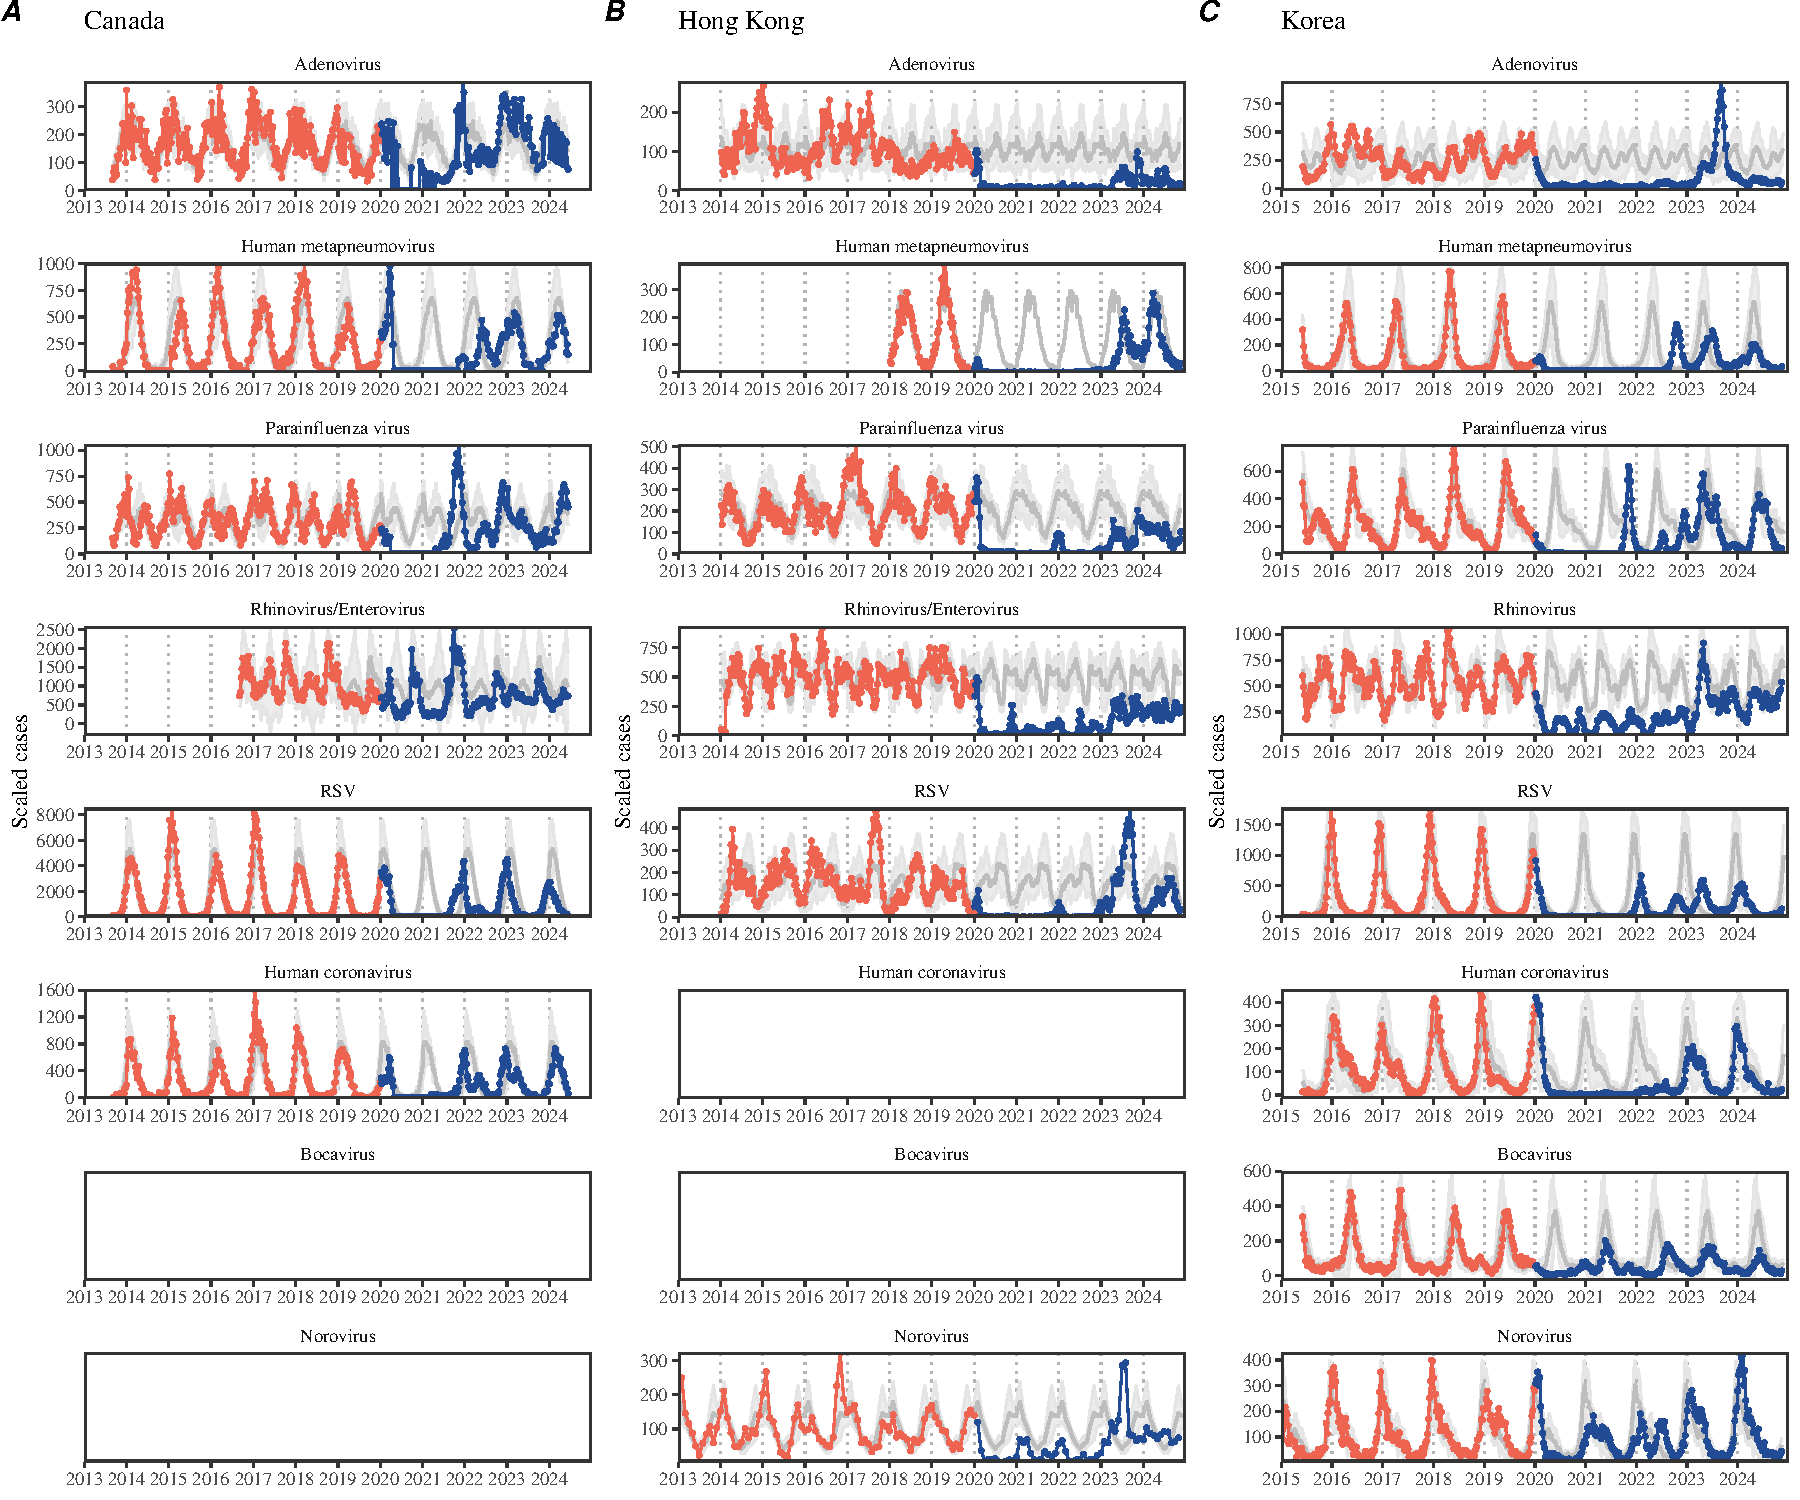
\includegraphics[width=\textwidth]{../figure1/figure1.pdf}
\caption{
\textbf{Observed heterogeneity in responses to COVID-19 pandemic across respiratory pathogens and norovirus in (A) Canada, (B) Hong Kong, (C) Korea, and (D) US.}
Red points and lines represent data before 2020.
Blue points and lines represent data since 2020.
Gray lines and shaded regions represent the mean seasonal patterns and corresponding 95\% confidence intervals based on the observed outbreak patterns before 2020.
}
\end{figure} 

To address this question, we propose a framework for characterizing the resilience of a host-pathogen system based on how fast the system recovers from perturbation.
We begin by laying out a few example scenarios that represent the expected outbreak dynamics following COVID-19 interventions and illustrating how resilience can be measured by comparing the post- and pre-pandemic dynamics of susceptible and infected hosts.
In practice, the dynamics of susceptible hosts are often unavailable, and traditional susceptible reconstruction approaches often require long-term endemic time series, which cannot be applied due to disruptions in epidemic patterns caused by COVID-19 NPIs.
Instead, we utilize Takens' embedding theorem to reconstruct empirical attractors from data and further measure the distance from this empirical attractor, which allows us to characterize the rate at which this distance decreases.
Analyses of pathogen surveillence data for a wide array of respiratory pathogens in Canada, Hong Kong, and Korea suggest ...
Finally, we show that variation in resilience estimates can be understood in terms of susceptible host dynamics.
\swp{Revisit.}
 
\section*{Conceptual introduction to pathogen resilience}

In classical ecological literature, resilience of an ecological system is measured by the rate at which the system returns to its reference state following a perturbation.
This rate corresponds to the largest real part of the eigenvalues of the linearized system near equilibrium---here, we refer to this value as the \emph{intrinsic} resilience of the system, which represents the expected rate of return from perturbated states.
However, respiratory pathogens often exhibit seasonal variation in transmission, meaning that the intrinsic resilience of a host-pathogen system varies across season.
Nonetheless, we can still measure the \emph{empirical} resilience of a host-pathogen system by looking at how fast the system returns to the pre-pandemic, endemic dynamics after interventions are lifted.

As an example, consider an intervention that reduce transmission by 50\% for 6 months starting in 2020, which causes epidemic patterns to deviate from its original stable annual cycle for a short period of time and eventually come back (Figure 2A).
To measure the empirical resilience of this system, we first need to be able to measure the distance from its pre-pandemic attractor.
There are many different ways we can measure the distance from attractor, but for illustrative purposes, we choose one of the most parsimonious approach: that is, we look at how the susceptible (S) and infected (I) populations change over time and measure the distance on the SI phase plane (Figure 2B).
In this simple case, the locally estimated scatterplot smoothing (LOESS) fit indicates that the distance from attractor decreases linearly on average (Figure 2C).
Furthermore, the overall rate of return matches the intrinsic resilience of the seasonally unforced system (Figure 2C).

\begin{figure}[!th]
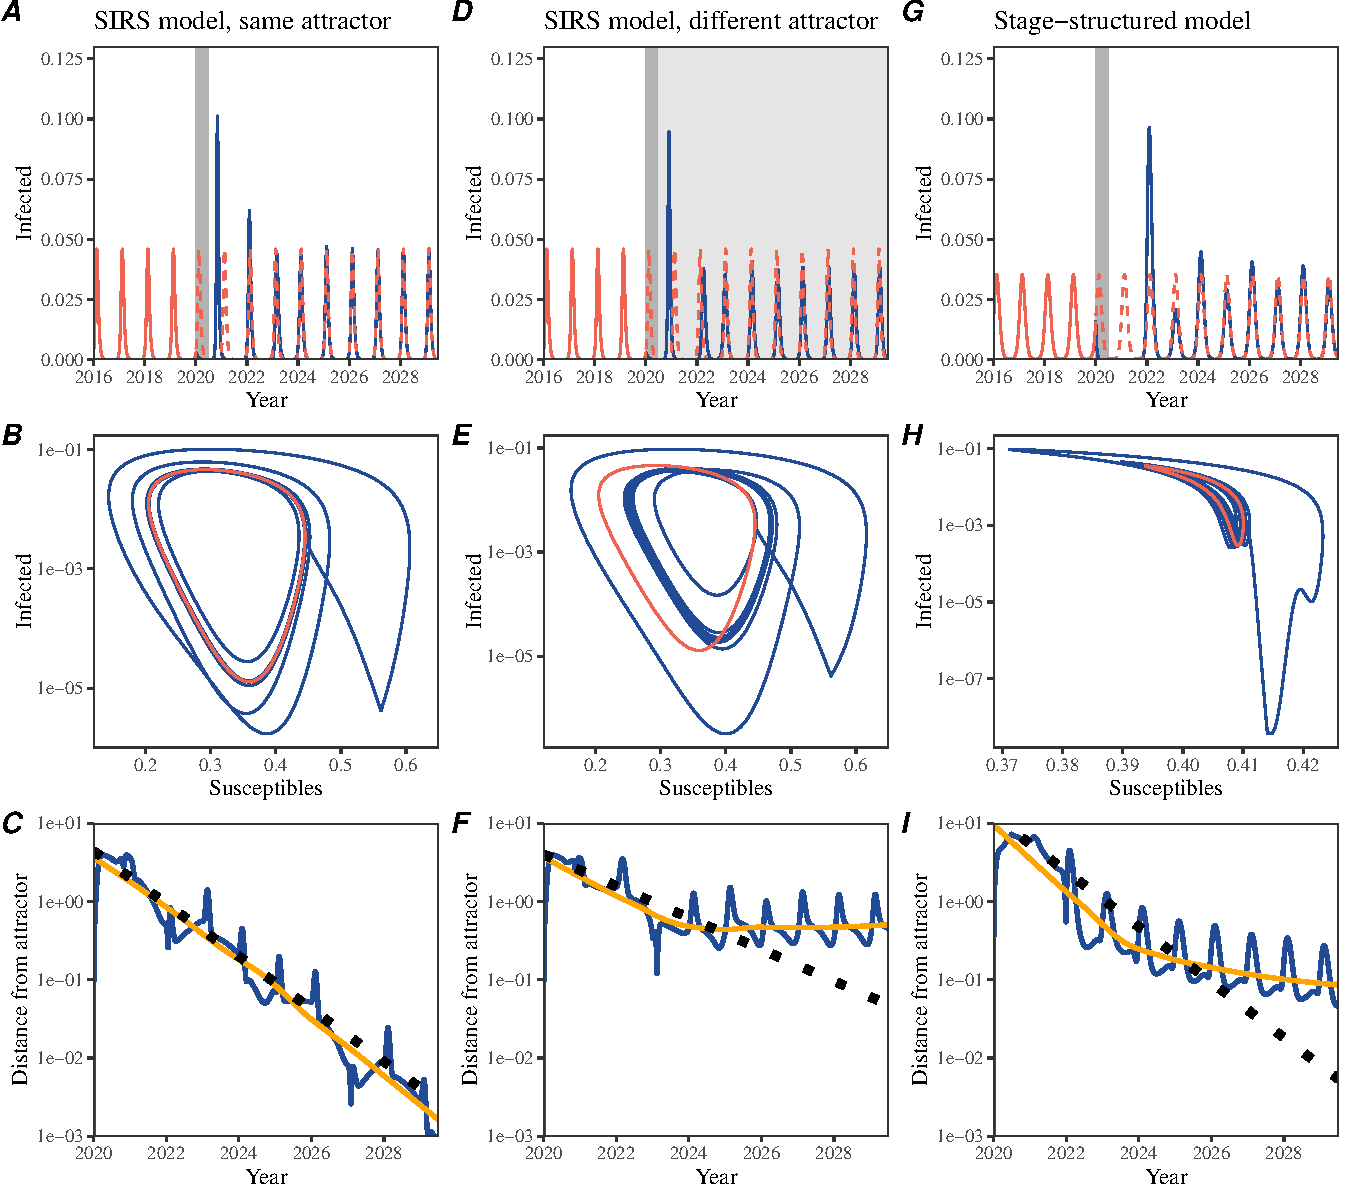
\includegraphics[width=\textwidth]{../figure2/figure2_simple.pdf}
\caption{
\textbf{Conceptual framework for measuring pathogen resilience following NPIs across different scenarios.}
(A, D, G) Simulated epidemic trajectories across various models. 
Red and blue solid lines represent epidemic dynamics before and after interventions are introduced, respectively.
Red dashed lines represent counterfactual epidemic dynamics in the absence of interventions.
Gray regions indicate the duration of interventions.
(B, E, H) Phase plane representation of the corresponding model.
Red and blue solid lines represent epidemic trajectories on an SI phase plane before and after interventions are introduced, respectively.
(C, F, I) Changes in logged distance from attractor over time.
Transparent solid lines represent the logged distance from attractor.
Non-transparent solid lines represent the locally estimated scatterplot smoothing (LOESS) fits to the logged distance from attractor.
Doted lines are superimposed as a comparison to have the same slope as the intrinsic resilience of the system.
}
\end{figure}

Alternatively, NPIs can permanently change our behavior and have persisting impact on the pathogen dynamics; 
as an example, we consider a scenario in which a 10\% reduction in transmission persists even after the NPIs are lifted (Figure 2D--F).
In such cases, we cannot know whether the pathogen will return to its original cycle or a different cycle until many years have passed after the NPIs are lifted, meaning that we cannot measure the distance against the new attractor that the system will eventually approach.
Nonetheless, we can still measure the distance against the original, pre-pandemic attractor and ask how the distance changes over time (Figure 2E).
The LOESS fit suggests that the distance from the attractor will initially decrease exponentially on average (equivalently, linearly on a log scale) and eventually plateau (Figure 2F).
Here, a permanent 10\% reduction in transmission rate slows down the system, which causes the distance from the attractor to decrease at a slower rate (Figure 2F) than it would have otherwise in the absence of permanent transmission reduction (Figure 2C).
This example shows that resilience is not necessarily an intrinsic property of a specific pathogen.
Instead, pathogen resilience is a property of a specific attractor that a host-pathogen system approaches, which depends on both pathogen and host characteristics.
\swp{Add discussion about observation error, e.g., under-reporting.}

Finally, transient phenomena can also complicate the picture (Figure 2G--I).
For example, a stage-structured model for RSV initially exhibits a stable annual cycle, but perturbations from NPIs cause the epidemic to exhibit biennial cycles (Figure 2G).
Despite this biennial cycle, we see that the system eventually approaches the original pre-pandemic attractor (Figure 2H), suggesting that this biennial cycle is a transient phenomenon.
The LOESS fit indicates that the distance from the attractor will initially decrease exponentially at a rate that is consistent with the intrinsic resilience of the seasonally unforced system, but the rate of decrease slows down as the epidemic exhibits a biennial cycle (Figure 2I).
In classical ecological theory, this behavior is also referred to as a ghost attractor, which causes long transient dynamics and slow transitions.

These observations indicate three possibilities.
First, we can directly estimate the empirical resilience of a host-pathogen system by looking at how fast the system approaches a pre-pandemic attractor, provided that we can measure the distance from attractor.
The empirical approach to estimating pathogen resilience is particularly convenient because it does not require us to know the true underlying model.
As we show in Supplementary Materials, estimating the intrinsic resilience from fitting standard compartmental models can lead to biased estimates, especially under model misspecification (\swp{TODO}).
Second, resilience estimates allow us to make phenomenological predictions about the dynamics of a host-pathogen system following a perturbation:
assuming that the distance from the attractor will decrease exponentially over time, we can obtain a ballpark estimate for when the system will reach an attractor.
Finally, deviation from an exponential decrease in the distance from attractor can provide information about whether the system has reached an alternative attractor, or a ghost attractor, that is different from the original, pre-pandemic attractor.
These alternative attractors may reflect continued perturbations from permanent changes in transmission patterns as well as changes in immune landscapes.

\swp{Multi-strain system to be discussed in the supp after some more investigation.}

\section*{Inferring pathogen resilience from real data}

Based on these observations, we now set out to infer pathogen resilience from real data.


\begin{figure}[!ht]
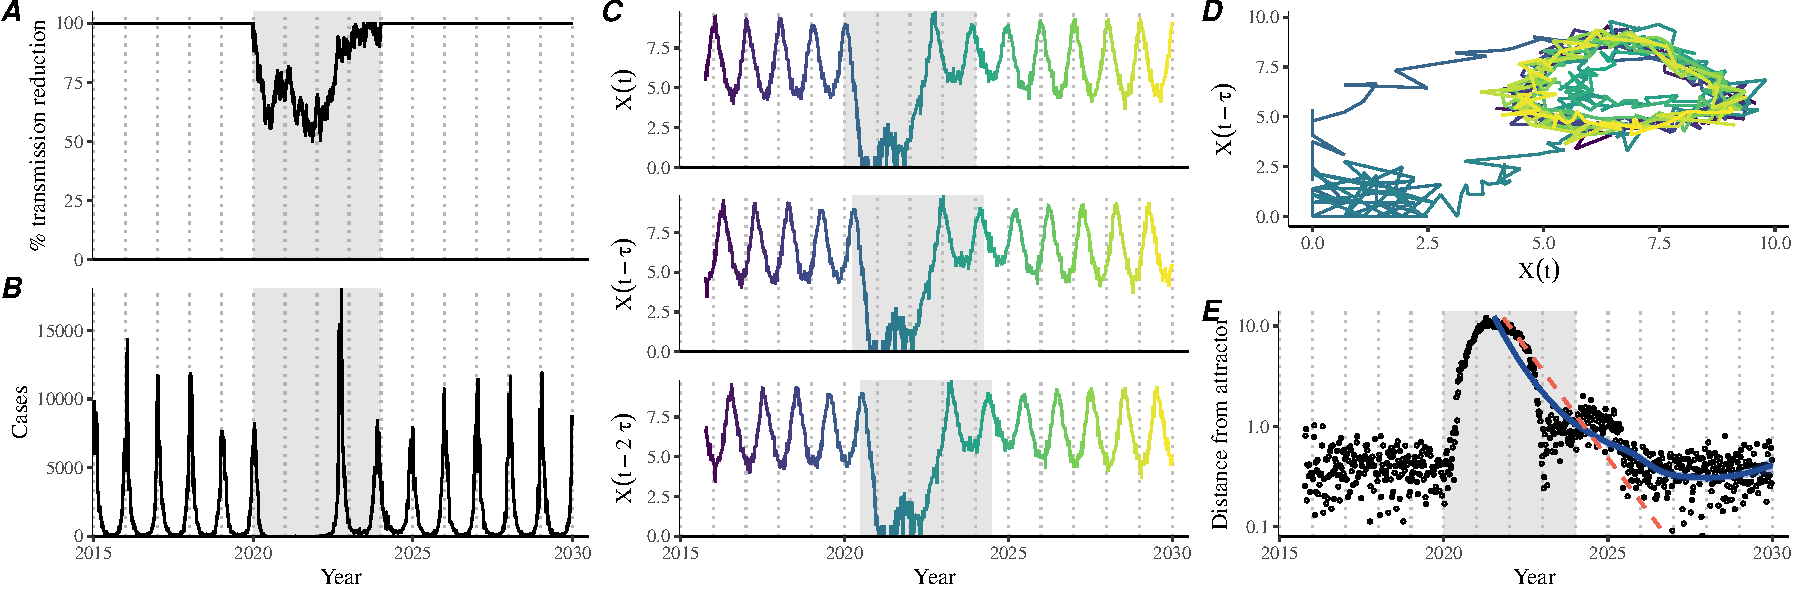
\includegraphics[width=\textwidth]{../figure_schematic/figure_schematic.pdf}
\caption{
\textbf{A schematic diagram explaining how pathogen resilience can be inferred from real data.}
(A) A realistic example of a synthetic NPI, represented by a relative reduction in transmission.
(B) The impact of the synthetic NPI on epidemic dynamics simulated using a stochastic SIRS model.
(C) Generating delayed copies of the logged time series allows us to obtain an embedding.
(D) Two dimensional representation of an embedding.
(E) Delayed embedding allows us to calculate the nearest neighbor distance from the empirical attractor, which is determined based on the pre-pandemic time series.
This distance time series can be used to infer pathogen resilience by fitting a linear regression after choosing an appropriate window for regression.
}
\end{figure}

To do so, we first reconstruct an empirical attractor by utilizing Takens' theorem, which states that an attractor of a nonlinear multidimensional system can be mapped onto a delayed embedding.
Here, we use delayed copies of logged values of pre-pandemic cases, $C(t)$, to reconstruct the attractor:
\begin{equation}
\langle\log(C(t)+1), \log(C(t-\tau)+1), \dots, \log(C(t-(M-1)\tau)+1)\rangle,
\end{equation}
where the delay $\tau$ and embedding dimension $M$ is determined based on autocorrelations and false nearest neighbors.
This allows us to measure nearest neighbor distance between the current state of the system and the empirical attractor at any given point in time, from which we can quantify how fast this distance decreases by fitting a linear regression on a log scale.
Then, the resulting estimate of the slope of linear regression corresponds to pathogen resilience.
Estimates of distance from attractor and linear regressions fits are presented in \swp{TODO: Supplementary Materials.}

For most pathogens, resilience estimates are consistent across different countries with a few exceptions (Figure 3A).
For example, resilience estimates for adenovirus for Hong Kong and Korea are orders of magnitudes lower than the corresponding estimate for Canada.
Another exception is human metapneumovirus, where the estimated resilience for Hong Kong is considerably higher than in other countries.
Otherwise, we find that resilience estimates range between 1--3/years for most other pathogens, suggesting a rather fast return to their regular outbreak cycles.

\begin{figure}[!th]
\begin{center}
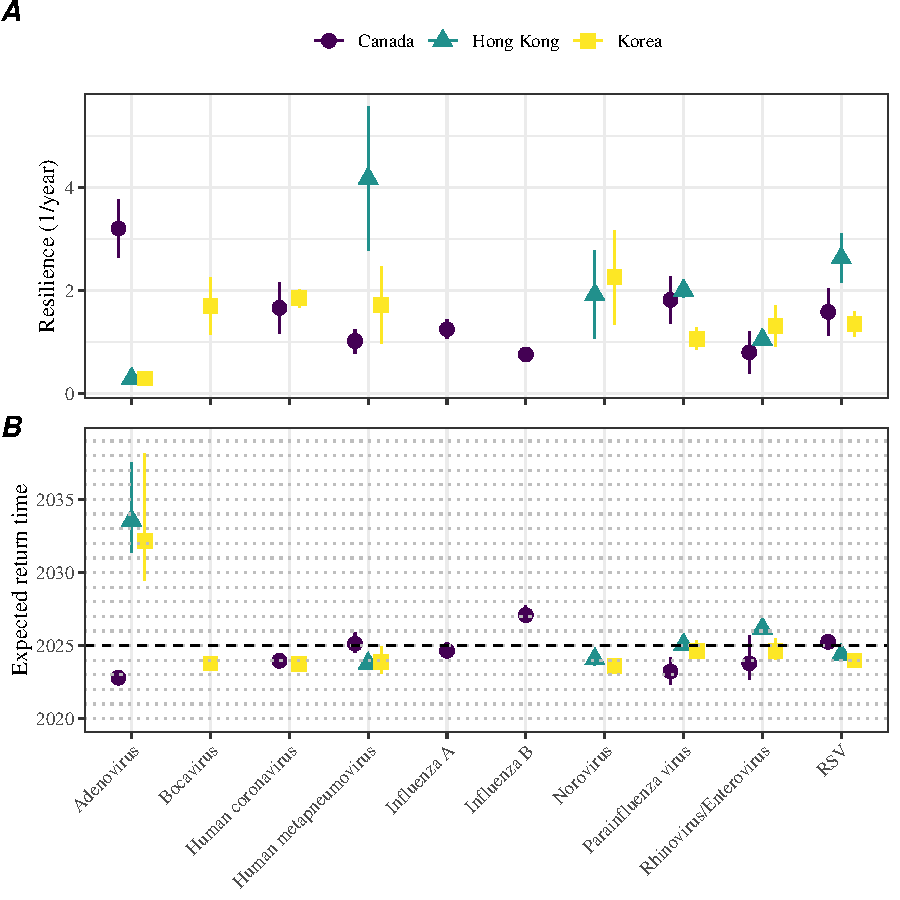
\includegraphics[width=0.8\textwidth]{../figure3/figure3.pdf}
\caption{
\textbf{Summary of resilience estimates.}
(A) Estimated pathogen resilience.
(B) Predicted timing of when each pathogen will return to their pre-pandemic cycles.
The dashed line in panel B indicates the end of 2024 (current observation time).
Error bars represent 95\% confidence intervals.
}
\end{center}
\end{figure}

Using resilience estimates, we now predict when each pathogen will return to their original pre-pandemic cycles.
Specifically, we extend our linear regression fits to empirical estimates of distance from attractor and ask when the predicted regression line will cross a threshold value, which we set to a mean of pre-pandemic distances.
Surprisingly, we find that most pathogens should have returned to their original cycles by the end of 2024 (Figure 3B).
While these predictions are consistent with several pathogens (e.g., seasonal coronavirus epidemics in Canada and Korea in Figure 1),
there are a few inconsistencies.
For example, we predict that bocavirus epidemics in Korea should have returned by the end of 2023 (Figure 3B), but the observed patterns indicate clear deviation from pre-pandemic cycles (Figure 1).
These deviations, alongside plateaus in the estimated distance from attractor, suggest that some of these pathogens, such as bocavirus, may have converged to different attractors.

\section*{Susceptible host dynamics explain variation in pathogen resilience}

So far, we focused on quantifying pathogen resilience from the observed patterns of pathogen re-emergence following COVID-19 interventions.
But what factors determine how resilient a host-pathogen system is?
Here, we use a standard Susceptible-Infected-Recovered-Susceptible (SIRS) model to show that susceptible host dynamics explain variation in pathogen resilience.
To do so, we vary the basic reproduction number $\mathcal R_0$, which represents the average number of secondary infections caused by a newly infected individual in a fully susceptible population, and the duration of immunity and compute intrinsic resilience for each parameter.

\begin{figure}[!th]
\begin{center}
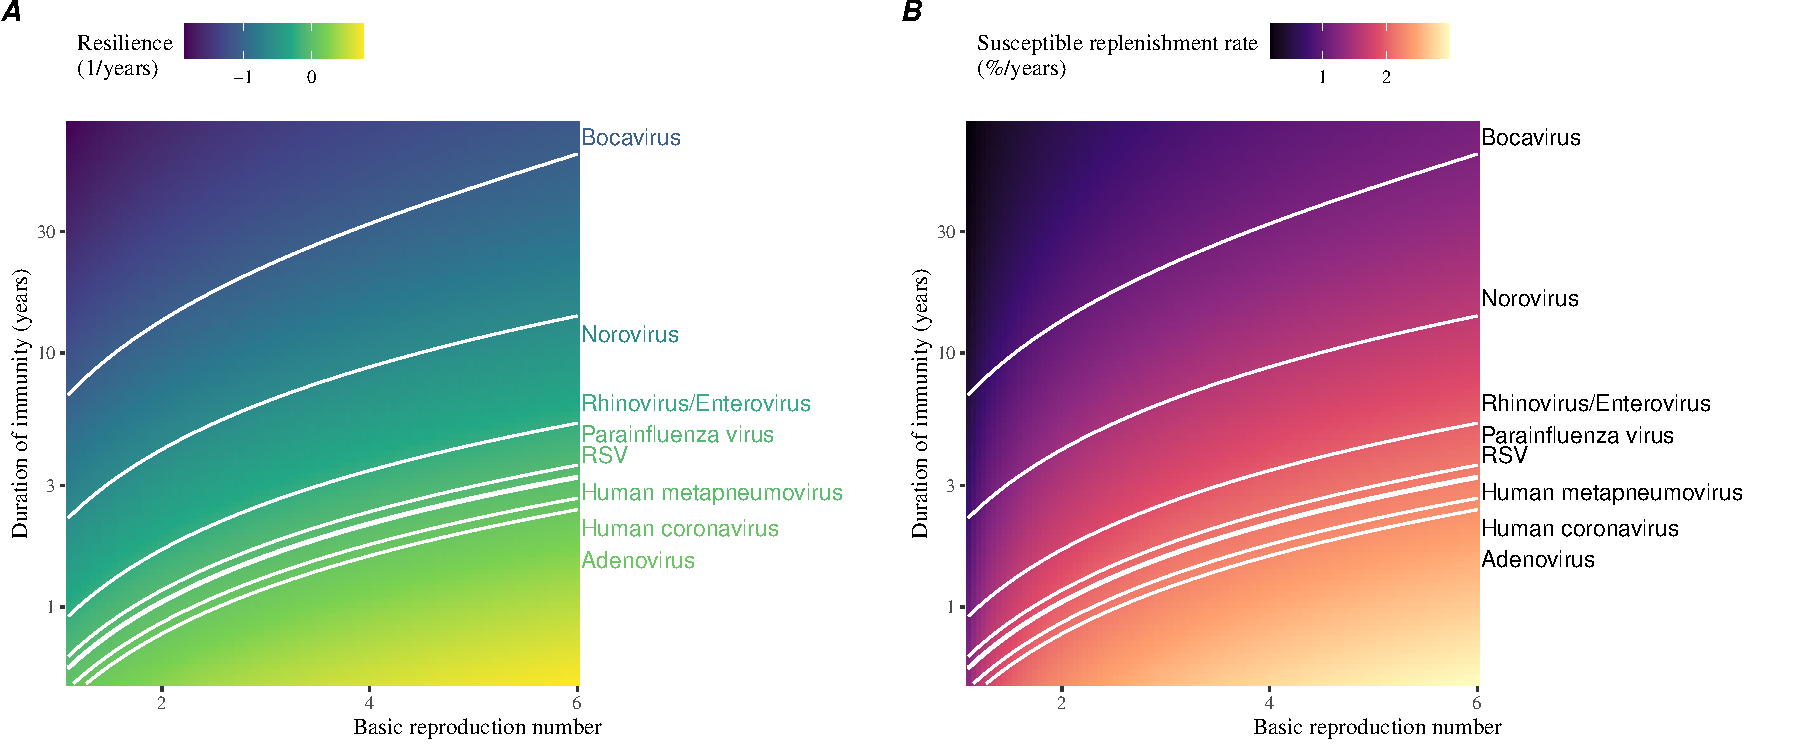
\includegraphics[width=\textwidth]{../figure_summary/figure_summary.pdf}
\caption{
\textbf{Linking pathogen resilience to epidemiological parameters and susceptible host dynamics.}
(A) The heat map represents intrinsic resilience as a function of the basic reproduction number $\mathcal R_0$ and the duration of immunity.
(B) The heat map represents per-capita susceptible replenishment rate as a function of the basic reproduction number $\mathcal R_0$ and the duration of immunity.
The standard SIRS model is used to compute intrinsic resilience and per-capita susceptible replenishment rate.
Lines correspond to a set of parameters that are consistent with mean resilience estimates for each pathogen.
Pathogens are ranked based on their mean resilience estimates, averaged across different countries.
}
\end{center}
\end{figure}

We find that pathogen resilience increases with higher $\mathcal R_0$ and shorter duration of immunity (Figure 4A).
These variations can be understood in terms of the susceptible host dynamics, where faster per-capita susceptible replenishment rate causes the system to be more resilient (Figure 4B).
This rate can be expressed as a ratio between absolute rate at which new susceptibles enter the population and the equilibrium number of susceptible individuals in the population, $\bar{S}$.
Therefore, both higher $\mathcal R_0$ and shorter duration of immunity can drive faster per-capita susceptible replenishment rate  (Figure 4B), especially because higher $\mathcal R_0$ leads to lower $\bar{S}$.

Finally, we can now rank different pathogens based on their empirical resilience.
For simplicity, we take the average of resilience estimates across countries to determine the ranking, which shows that influenza B is least resilient (Figure 4A).
This observation is consistent with the extinction of influenza B/Yamagata, which indicates the persistence of a pathogen should be associated with its resilience.
Similarities in resilience ranking between RSV and Human metapneumovirus is also interesting, given the apparent coupling of their dynamics through cross immunity.
These rankings further allow us to map each pathogen onto a set of parameters that are consistent with its empirical resilience (Figure 4A) and obtain a plausible range of susceptible replenishment rates for each pathogen (Figure 4B).

\section*{Discussion}

The COVID-19 interventions have caused major disruptions to circulation patterns of both respiratory and non-respiratory pathogens, adding challenges to predicting their future dynamics.
On the other hand, these interventions offer large-scale natural experiments for understanding how different pathogens respond to perturbations.
In this study, we show that pathogen re-emergence patterns following COVID-19 interventions can be characterized through the lens of ecological resilience.
Traditionally, ecological resilience measures how fast a system returns to a reference state following a perturbation.
In the context of respiratory pathogens, resilience measures how fast epidemics return to their endemic cycles after interventions are lifted.
% Our study demonstrates that this perspective provides unique insights into underlying susceptible host dynamics and allows predictions for when epidemics will return to their endemic cycles.

We use an attractor reconstruction approach to quantify how distance from attractor changes over time for each pathogen.
By fitting a linear regression to log distances, we can estimate pathogen resilience and further predict when each pathogen will return to their endemic cycles.
Consistency in resilience estimates across countries is particularly surprising given that each country imposed different intervention measures; this consistency provides robustness to our estimates.
The ability to predict future epidemic patterns from resilience estimates also offers a new paradigm for epidemic forecasting.
While this approach cannot predict the exact timing of outbreaks or epidemic patterns, it is nonetheless useful for predicting when epidemics will settle down to regular cycles after a large perturbation, such as COVID-19 interventions.

Our analyses suggest a possibility that several pathogens may have converged to different endemic cycles compared to their pre-pandemic epidemic patterns.
Key examples include human metapnuemovirus, RSV, and bocavirus in Korea as well as RSV in Hong Kong.
These changes may reflect permanent changes in behavior since 2020 or a shift in population-level immunity.
However, it seems unlikely that permanent changes in behavior would only affect a few pathogens and not others.
A shift in population-level immunity is plausible, as the emergence of SARS-CoV-2 and extinction of influenza B/Yamagata likely caused major changes in immune landscapes;
however, we currently do not know how immunity, or lack thereof, from these pathogens would affect infection from other pathogens.
Future studies should use detailed mechanistic models, coupled with behavioral and immunological data, to test these hypotheses and better understand post-pandemic dynamics of endemic pathogens.

We show that susceptible host dynamics shape pathogen resilience, where faster replenishment of the susceptible population causes the pathogen to be more resilient.
For simplicity, we focus on waning immunity and birth as a main driver of the susceptible host dynamics but other mechanisms can also contribute to the replenishment of the susceptible population.
In particular, pathogen evolution, especially the emergence of antigenically novel strains, can cause effective waning of immunity in the population;
therefore, we tentatively hypothesize that faster rates of antigenic evolution can also cause a pathogen to be more resilient.
Future studies should explore the relationship between the rate of evolution and resilience for antigenically evolving pathogens.

Quantifying pathogen resilience also offers novel approaches to validating epidemiological models.
So far, the majority of model validation in epidemiology is based on the ability of a model to reproduce the observed epidemic dynamics and to predict future dynamics.
However, there can be plethora of models that meet these criteria.
For example, two major RSV models have been proposed so far to explain biennial epidemic patterns: (1) a stage- and age-structured model that allows for disease severity to vary with number of past infections and age of infection and (2) a pathogen-interaction model that accounts for cross immunity between RSV and human metapnuemovirus.
Since both models can accurately reproduce the observed epidemic patterns, standard criteria for model validation do not allow us to distinguish between these two models.
Instead, we can measure the empirical resilience of each model by simulating various perturbations and compare them to estimates of empirical resilience from data, using COVID-19 interventions as an opportunity.
Future studies should further investigate using pathogen resilience for validating epidemic models.

There are several limitations to our work.
In particular, our estimates of pathogen resilience and the associated ranking are necessarily crude.
\swp{Limitation TBD.}
Nonetheless, our study illustrates the utility of quantifying pathogen resilience for understanding how different pathogens respond to perturbations.

\swp{Conclusion paragraph TBD.}

\section*{Materials and Methods}

\subsection*{Data}

We gathered time series on respiratory infections from four different countries: Canada, Hong Kong, Korea, and United States (US).
As a reference, we also included time series data on norovirus infections for available countries---in contrast to respiratory pathogens, we expect gastrointestinal viruses, such as norovirus, to be less affected by COVID-19 intervention measures.

Weekly time series of respiratory infection cases in Canada come from the Respiratory Virus Detection Surveillance System, which collect data from select laboratories across Canada.
We extracted the data from \url{https://www.canada.ca/en/public-health/services/surveillance/respiratory-virus-detections-canada.html}.

Weekly time series of respiratory infection cases in Hong Kong came from the Centre for Health Protection, Department of Health. 
We extracted the data from \url{https://www.chp.gov.hk/en/statistics/data/10/641/642/2274.html}.

Weekly time series of respiratory infection cases in Korea came from Korea Disease Control and Prevention Agency.
We extracted the data from \url{https://dportal.kdca.go.kr/pot/is/st/ari.do}.

Finally, weekly time series of respiratory infection cases in the US comes from the National Respiratory and Enteric Virus Surveillance System.



\pagebreak

\bibliography{return-time.bib}

\end{document}
